\documentclass[12pt,onecolumn,twoside]{article}
\usepackage[T1]{fontenc}
\usepackage[utf8]{inputenc}
\usepackage{amsfonts, amsmath}
% \usepackage{nature}
\usepackage{wrapfig}

\usepackage{cell}
\usepackage{natbib}
% The Cell style only works with BibTeX and not BibLaTeX. So load the 'cell' package here, the bib and style file commands in the document at the end, and make sure the cell.bst file is in the same directory as the tex file. Once all of this is in place, compile on the terminal with this sequence: xelatex filename, bibtex filename.aux, xelatex filename, xelatex filename. Atom-latex is a bit unreliable in this regard.

\usepackage[document]{ragged2e} %For non-justified text alignment
\usepackage[margin=0.75in]{geometry}
\usepackage{fontspec}
\setmainfont{Carlito}
\usepackage{hyperref}
\hypersetup{
	colorlinks = true, %Colours links instead of ugly boxes
	urlcolor = blue, %Colour for external hyperlinks
	linkcolor = red, %Colour of internal links
	citecolor = blue %Colour of citations
}
%\usepackage{threeparttable}
\usepackage{graphicx}
\usepackage{caption}
\usepackage{subcaption}
% \usepackage{fancyhdr}
% \pagestyle{fancy}
% \fancyhf{}
% \rhead{\thepage}
% inkscape -D image.svg  -o image.pdf --export-latex is the command for SVG to TeX export
\makeindex

\usepackage{authblk}
\author{Vibishan B.}
\affil{Department of Biology, Indian Institute of Science Education and Research (IISER), Pune}

\title{Annual meeting of the RAC}
\date{8 July, 2021}

\begin{document}
	\maketitle
	\section{Dispersal selection line-progress so far}
	In reference to the report submitted to this committee in June 2020, selection for dispersal in lab populations of the fruit fly, \textit{Drosophila melanogaster} was intended to be a central part of my thesis work. Specifically, I proposed to continue an ongoing investigation into the evolution of dispersal in fruit fly populations under conditions of larval malnutrition. In this selection regime, flies were selected for development on larval food with reduced dietary protein in addition to selection at the adult stage for ambulatory dispersal. It was expected that the dual selection pressure of evolving higher dispersal following development under malnutrition would manifest costs of adaptation that were not apparent in dispersal evolution in normal dietary conditions. At the time of writing the report last year, 45 generations of selection had been carried out in four replicate populations (blocks)-each large and outbred of about 2400 flies-and assays had been performed at generation 42 to look for an adaptive response. I had found that flies selected for dispersal and malnutrition (MD-\underline{M}alnourished \underline{D}ispersers) initiated dispersal to a greater extent and dispersed over longer distances than the corresponding control populations (MC-\underline{M}alnourished \underline{C}ontrol). While this tendency towards higher dispersal was corraborated by higher locomotor activity and fewer bouts of rest (measured using the Drosophila Activity Monitor, DAM) in the MD populations than MC, I had not detected any cost of this adaptive response in dry body weight or fecundity.

	\paragraph{\empty}The dataset at the time was incomplete since the fecundity measurement had to be repeated for two of the four blocks. Further followup assays were also planned to measure changes in behavioural traits including male-male aggression and exploration, as well as in dessication and starvation resistance. %The choice of these behavioural traits follows directly from the observation of higher locomotor activity in MD, while both dessication and starvation resistance serve as readouts of stress tolerance capacity which could be an important aspect of life history strategy, particularly when nutrition selection is involved.%
	All of these plans were interrupted by the Covid-19 pandemic and the consequent campus lockdown. Selection for dispersal in the MD populations had to be suspended from March to November 2020, spanning 11 generations of relaxed selection. Before resumption of selection therefore, measurements were made of dry body weight and locomotor activity to assess the extent, if any, of the loss of phenotype due to relaxation. The locomotor activity phenotype was largely preserved, and MD males remained more active and rested less than MC males. On the other hand, the trends in body weight were inconsistent with the pre-pandemic data; where earlier there were no clear differences between MD and MC, both MC females and males were consistently heavier than corresponding MD flies in the post-lockdown measurement. A visual comparison with the older data suggests that MC flies in particular may have gotten heavier while MD flies have stayed roughly the same, but this comparison has not been made quantitatively. As the locomotor phenotype has remained demonstrably similar, I have since resumed selection for malnourished dispersal in MD-nearly 20 more generations of selection have been carried out and we are now at 62 generations of selection completed.

	\paragraph{\empty}Given the inconsistencies in the body weight data before and after the lockdown, the generation 42 experiments will need to be repeated to confirm the adpative change in dispersal properties and to clarify the actual trends in body weight alongside. However, current manpower limitations at the lab present logistic hurdles to planning large-scale experiments, and I therefore plan to conduct smaller experiments instead that can be carried out with fewer people. This includes physiological measurements like glucose and triglyceride content. It is possible that the DAM setup used for measuring locomotor activity can also provide indirect readouts of time to dessication and I plan to explore this possibility. A protocol for measuring food consumption rates based on uptake of a coloured dye is also nearing complete standardisation and can therefore add to a smaller-scale experimental investigation of the evolution of malnourished dispersal in the next month or two. Larger experiments like the dispersal kernel will have to be done one block at a time over a longer period of time.

	\section{Theoretical investigations in cancer}
	This new line of study was initiated around August 2020 and consists of the following distinct subjects of inquiry.

	\subsection{Adaptive therapy}
	Among numerous recent developments in cancer treatment strategies, one which holds particular interest for ecologists is adaptive therapy. The conventional chemotherapy paradigm that is currently in practice involves a cytotoxic drug which is administered at, or close to, the maximum tolerated dose (MTD) in order to maximise the number of tumour cells killed by the drug. However, cancer cell populations are known to be highly heterogeneous in their genotypes and phenotypes \citep{DENTRO20212239, Shen2020a, Geiler-Samerotte2013, Hu2016}, and this heterogeneity can often engender smaller, subclonal populations within a growing tumour that may already be resistant to a cytotoxic drug. Consequently, when the drug is administered at MTD to maximise cell kill, the sensitive fraction of the cancer population is all but eliminated, freeing up space and resources for the resistant clones to grow into. Such competitive release clearly has key implications for tumour relapse and the clinical development of drug resistance, and the fundamental goal of adaptive therapy is to delay or prevent such competitive release of resistant cells \citep{Gatenby2009}. Cancer cell populations are known to accommodate a range of ecological interactions among subclonal populations \citep{KotlerBrown2020}-competition particularly prominent among them \citep{Parker2020}-and adaptive therapy involves administering lower, fluctuating doses of the cytotoxic drug, such that some fraction of drug sensitive cells remain in the tumour population to inhibit through biotic competition, the growth of resistant cells. The dosage schedule is responsive to changes in the tumour burden-if the burden exceeds a set upper threshold, the drug is given until the burden falls below a lower threshold, after which it is withdrawn. This leads to a therapy paradigm that treats to maintain controllable tumour growth as opposed to the conventional treat-to-cure approach \citep{Hansen2017a, Hansen2020a}.

	\paragraph{\empty}Late-stage castration-resistant prostate cancer has seen the most progress in terms of theoretical development of adaptive therapy protocols \citep{Cunningham2018, West2018b, Jain2011} as well as direct application in a recent pilot clinical trial \citep{Zhang2017a}. This system has been modelled as a combination three cell types. The baseline prostate cancer population consists of cells that are dependent on the androgen, testosterone for their growth-these cells are called $T^+$ and since they are dependent on external supply of testosterone, they are sensitive to chemical castration using antiandrogens. During cancer progression, mutations have been demonstrated that allow cancer cells to repurpose existing metabolic pathways to produce their own testosterone-these cells are called $T^p$ (producers of testosterone) and they are insensitive to chemical castration. Testosterone produced and secreted by $T^p$ is a common resource that used by both $T^p$ and $T^+$, and this production can be inhibited by targeted drugs like abiraterone which is currently the frontline treatment for castration-resistant prostate cancer. A third cell type can also arise by mutation that allows for testosterone-independent growth by modifications to the androgen receptor making them constitutively active-these cells are collectively called $T^-$, and they are insensitive both to chemical castration and to inhibitors like abiraterone that target testosterone production, making them impossible to treat with a castration-abiraterone regimen.

	Working with an undergraduate student, I formulated this sytem into a three-species ODE model based on a Lotka-Volterra framework, with additional equations describing the dynamics of one public resource that is used by all three cell types (oxygen, in this case) and one partly private resource that is shared by two of the cell types (testosterone, labelled $T$). Castration-resistant tumours typically develop following androgen ablation which knocks out external production of testosterone and all testosterone in the system is therefore produced by $T^p$ with no bulk supply from systemic testosterone production. Oxygen is modelled entirely as a bulk supply term from the bloodstream. Data from \textit{in vitro} cell lines corresponding to each of the cell types were used to parameterise growth and death rates, as well as some resource consumption terms.\\

	The ODEs for population size of a cell type, $y_i$ includes the growth rate, $r_{i,max}$ and the death rate, $\delta_i$ (equation \ref{cell_eq}). The effective carrying capacity in the denominator varies between 1 to $K_{i,max}$ depending upon resource availability. This dependence was encoded as a function of the form given by equation \ref{fres_eq} and visualised in Figure \ref{fig_fres}.\\
	For $i \in \{T^+,T^p,T^-\}$
	\begin{equation}
	  \frac{dy_i}{dt} = r_{i,max} y_i (1 - \frac{\sum_j y_j}{1 + K_{i,max} f_i(O_2) f_i(T)} )- \delta_i y_i
	  \label{cell_eq}
	\end{equation}

	For $R \in \{O_2,T\}$
	\begin{equation}
	  f_i(R) = \begin{cases}
	  1 &\text{if } ul_{R,i} \leq R \\
	  \frac{R-ll_{R,i}}{ul_{R,i}-ll_{R,i}} &\text{if } ll_{R,i} < R < ul_{R,i} \\
	  0 &\text{if } R \leq ll_{R,i} \\
	  \end{cases}
	  \label{fres_eq}
	\end{equation}

	\begin{wrapfigure}{r}{0.5\textwidth}
	% \begin{center}
		\centering
		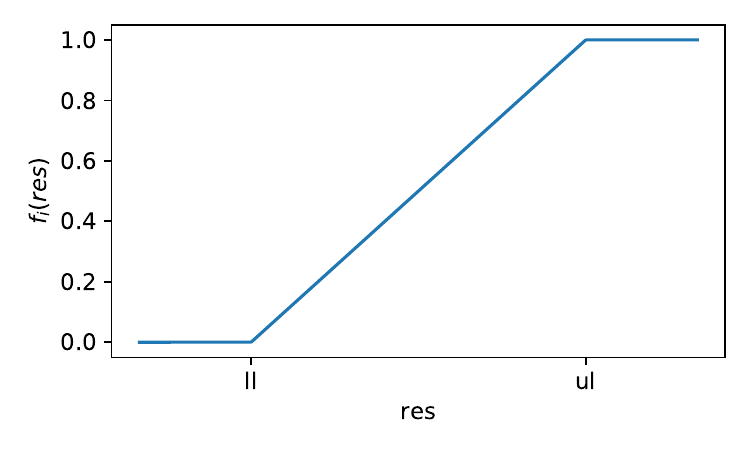
\includegraphics[width=0.3\textwidth]{f_res}
	% \end{center}
	\caption{\small Functional response, $f_i(R)$, for cell type $i$ against the concentration of the resource, $R$; this value modifies the carrying capacity in equation \ref{cell_eq}.}
	\label{fig_fres}
	\end{wrapfigure}

	The primary aim of this model was to study the dynamics of competition between the three cell types operating through resource dynamics. Coexistence between the drug sensitive and resistant cell types has obvious implications for therapeutic success, as a largely $T^-$ cell population would be highly unresponsive and therefore, not very treatable. Therapeutic success in the model can be defined based on two qualitative features-whether the model tumour population is responsive to treatment with abiraterone, and whether there are any treatment schedules that can successfully reduce the total tumour burden.

	\paragraph{\empty}Results from the model have shown that although $T^-$ has the shortest doubling time, the final outcomes of competition among the various cell types can be tuned considerably based on their resource response functions, $f_i(R)$. Under the right combination of sensitivities to resource limitation, $T^-$ could be outcompeted by the other two cell types which has important consequences for therpeutic resistance. The model can also be used to demonstrate that a tumour with a predominantly $T^p-T^+$ population is more responsive to abiraterone treatment (data not shown). We have still not been able to find a dosing regimen that can bring down the total tumour burden without losing responsiveness.
	\begin{figure}
	\centering
		\includegraphics[width=\textwidth]{fig2}
		\caption{\small Final ratios of the three cell types after 1000 days of simulated dynamics. ``no", ``low", and ``moderate" are levels of resource limitation that are modelled by setting suitable values of upper limit, $ul_{R,i}$ and lower limit, $ll_{R,i}$ in the function $f_i{R}$ (equation \ref{fres_eq}); columns correspond to oxygen limitation while rows correspond to testosterone limitation. The initial seeding ratios of the three cell types are shown above the figures in the order $T^p$:$T^+$:$T^-$, and three different total population sizes-plotted on the x-axis as total initial seeding-were run for each seeding ratio. The data demonstrates that resource limitations can clearly supersede differences in doubling times to determine the final outcome of competition; doubling times scale in this order: $T^- < T^+ < T^p$.}
	\end{figure}

	Taken together, the indications so far lead to three possible avenues of further development, all of which are being pursued actively in conjunction with summer students from IISER Pune:
	\begin{enumerate}
		\item The particular use of the carrying capacity term in equation \ref{cell_eq} is unusual, and to the best of my knowledge, unprecendented. Notwithstanding potential mathematical flaws in such an approach, a true consumer-resource model that does not have an explicit carrying capacity term is a better-understood, and arguably more established, way of modelling population growth as a result of resource dynamics, and one such model is being formulated now. It might also be interesting to evaluate the performance of the consumer-resource model against that of the existing model (equation \ref{cell_eq} and \ref{fres_eq}), towards a more systematic understanding of the roles of carrying capacities in models of population ecology.
		\item As mentioned earlier, the treatment protocols tried with the current model were successful in terms of maintaining a responsive tumour but unsuccessful in terms of reducing total tumour burden. A closer study of protocol design is now being considered to expand our exploration of the parameter space. This is planned to include the population size window that determines the on-off rules for therapy, frequency of drug administration, and multi-drug combination treatments, all of which are part of the optimisation process in present-day clinical trials as well as approved treatment methods.
		\item Solid tumours are generally spatially-complex systems with stark gradients in resources, signalling molecules, pH, and other biochemical substrates and side-products of a wide range of metabolic processes. It is well-known that solid tumours run out of oxygen and nutrients, especially in their centres, as they outgrow local blood supply and continue to expand. Such gradients lead to ennvironmental heterogeneity that can have significant effects on therapeutic outcomes and models can be developed, either as an agent-based framework or as a discretised reaction-diffusion system, to elucidate how competitive outcomes shift when spatial dynamics are added to the model. At the moment, we are developing the latter framework as the working model for spatial dynamics as numerical methods provide a relatively inexpensive way to describe large parts of model behaviour.
	\end{enumerate}

	\subsection{Models of cancer incidence}
	Patterns in cancer incidence can be stratified broadly in two levels:
	\begin{enumerate}
		\item Across several vertebrate taxa, cancer incidence is seen not to be correlated with body size or life span \citep{Peto2015}, which is surprising. Having a larger body and/or having to sustain somatic tissue for a longer period of time would both be expected to increase the risk of cancer; larger bodies require more cells and more cell division cycles to produce and maintain, while longer lifespans entail potentially higher cell turnover due to environmental damage or regular wear-and-tear. A wide range of theories and explanations have been proposed to address this apparent contradiction and some instances of taxon-specific cancer preventive genetic features have been found \citep{Abegglen2015, Tian2013, Gorbunova2014}. On the other hand, some aspects of the process of somatic mutation itself remain unaddressed. Importantly, most models of cancer incidence across species consider somatic (non-germline) mutations happening within the lifetime of an organism as effectively neutral, even though cancer progression is demonstrably a process of somatic evolution that involves selection on intermediate mutant clones \citep{Nowell1976}. It would be interesting to consider how change in cell number or lifespan affects cancer risk if the selective effects of somatic clones are included in the analysis.
		\item Within the same species, population-level incidence trends with age also hold interest. More specifically, data from human populations in the US show that cancer incidence begins to rise near the middle of life, reach a distinct peak around 70 years of age and then decrease in the oldest age classes \citep{Harding2012}. The decrease later in life is particularly interesting and so far, it is not entirely clear how it occurs or if there are any parallels to the well-known late-life mortality plateaus seen in humans and dipterans \citep{Mueller15249}. The processes underlying the late-life decline in cancer incidence could therefore be the subject of theoretical study, but this remains tentative.
	\end{enumerate}

	I am pursuing both these possibilities with a Master's student from IISER Pune. We spent the last semester developing an agent-based simulation framework using a recently published agent-based model \citep{Erten2020} as a template. This published model provided a starting point from which we have built a simpler, pared-down model that can be used to address the process of mutation accumulation with age more specifically. We are now trying to generate predictions regarding the variation of cancer risk with cell number and patterns in cell turnover while also accounting for selection processes that could be operating at the somatic level.

	\section{Timeline}
	The move to fly work in 2019 and the pandemic-induced suspension have both added delays to the timeline of completion. In this report, I have laid out several lines of work that are expected to be part of my thesis eventually, but their satisfactory execution and completion is likely to take another year still and would therefore require an extension of my PhD tenure.

	\bibliographystyle{cell}
	\bibliography{review}
	% \printbibliography

\end{document}
